\usetikzlibrary{automata,arrows}

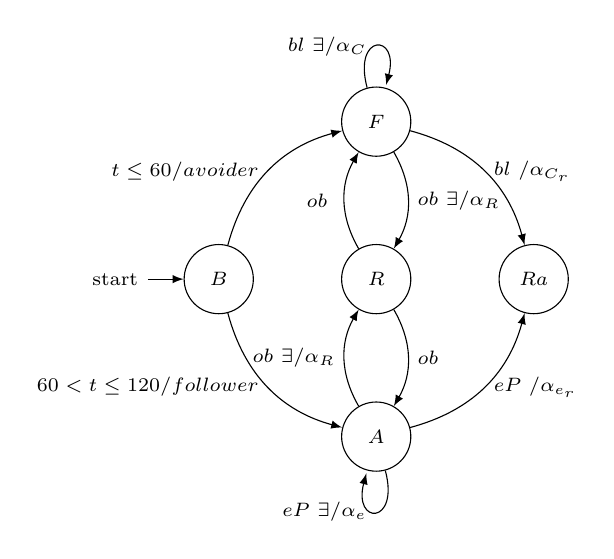
\begin{tikzpicture}[font=\scriptsize, ->, >=latex, node distance=2cm]
	\node[state, initial] (B) {$B$};
	\node[state, right of=B] (R) {$R$};
	\node[state, above of=R] (F) {$F$};
	\node[state, below of=R] (A) {$A$};
	\node[state, right of=R] (Ra) {$Ra$};
	\path   		
		(B) edge[bend left, left] node{$t\leq 60/avoider$} (F)		
		(B) edge[bend right, left] node{$60<t\leq 120/follower$} (A)		
		(R) edge[bend left, left] node{$ob~\nexists$} (F)
		(R) edge[bend left, right] node{$ob~\nexists$} (A)
		(F) edge[loop above, left] node{$bl~\exists/\alpha_C$} (F)
		(F) edge[bend left, right] node{$ob~\exists/\alpha_R$} (R)
		(F) edge[bend left, right] node{$bl~\nexists/\alpha_{C_r}$} (Ra)
		(A) edge[bend left, left] node{$ob~\exists/\alpha_R$} (R)
		(A) edge[bend right, right] node{$eP~\nexists/\alpha_{e_r}$} (Ra)
		(A) edge[loop below, left] node{$eP~\exists/\alpha_e$} (A)
	;	
\end{tikzpicture}
